\documentclass[10pt,twocolumn,letterpaper]{article}

\usepackage[letterpaper, top=0.9in, bottom=0.9in, left=0.75in, right=0.75in,
            columnsep=0.3in]{geometry}
\usepackage{times}
\usepackage{amsmath}
\usepackage{amssymb}
\usepackage{booktabs}
\usepackage{graphicx}
\usepackage{microtype}
\usepackage[numbers,sort&compress,square]{natbib}
\usepackage[hidelinks]{hyperref}
\usepackage{caption}
\usepackage{titlesec}

\captionsetup{font=small, labelfont=bf, skip=4pt}
\titleformat{\section}{\normalfont\large\bfseries}{\thesection.}{0.5em}{}
\titleformat{\subsection}{\normalfont\normalsize\bfseries}{\thesubsection.}{0.5em}{}
\titlespacing*{\section}{0pt}{0.8ex plus 0.3ex minus 0.2ex}{0.4ex plus 0.2ex}
\titlespacing*{\subsection}{0pt}{0.6ex plus 0.2ex minus 0.2ex}{0.3ex plus 0.2ex}

\setlength{\parskip}{0.15em}
\setlength{\parindent}{1.0em}

\title{Evidence-Blindness in Multimodal Medical Claim Verification:\\
       A Counterfactual Diagnostic and Training-Time Mitigation}
\author{Aayan Alwani\textsuperscript{1} \quad Ethan Wang\textsuperscript{2}}
\date{}

\begin{document}

\twocolumn[
  \begin{@twocolumnfalse}
  \maketitle
  \begin{abstract}
  \noindent
  Multimodal claim verifiers are used as safety layers after chest-X-ray report generators, and recent systems report above 90\% AUROC on hallucination-detection benchmarks. We show those numbers can be reached by a verifier that never looks at the image. We call this failure mode \emph{evidence-blindness}. To test for it, we alter a verifier's input in three ways at evaluation time and measure how much accuracy drops: zero out the image (image-masking gap, IMG); shuffle the retrieved evidence text across claims (evidence-shuffling gap, ESG); flip the image left to right on claims that hinge on side (image-perturbation gap, IPG). The diagnostic catches an immediate trap: the verifier with the highest validation accuracy we trained is fully evidence-blind (IMG $= 2.17$pp at validation accuracy $0.911$). A consistency loss combined with an adversarial hypothesis-only filter lifts IMG from $2.03$pp to $69.24$pp at $92.5\%$ test accuracy. The fix is brittle: under leave-one-site-out training, IMG regresses to $3.21$pp on held-out OpenI, and the same three metrics catch the regression --- so the diagnostic doubles as a deployment-shift alarm. Wrapping inverted conformal selection around each verifier reveals one further consequence: every evidence-blind configuration produces an empty trusted set, while only the non-blind verifier yields a populated set of $985$ claims at $\alpha = 0.10$ with FDR $0.91\%$. A conformal guarantee on a blind verifier has nothing to certify.
  \end{abstract}
  \vspace{0.6em}
  \end{@twocolumnfalse}
]

\section{Introduction}
\label{sec:intro}

Radiology report generation has moved from a demonstration task to a near-deployment tool. Systems such as MAIRA-2 \citep{bannur2024maira2}, CheXagent-2 \citep{chen2024chexagent}, and MedGemma \citep{google2025medgemma} produce structured findings reports from chest radiographs that are beginning to reach radiologists' review queues as first drafts, with reported hallucination rates of $8$--$15\%$ \citep{zhang2024radflag,hardy2024rextrust}. The community's response is to insert a claim-level verifier downstream of the generator. Recent verifiers report AUROC above $90\%$ on aggregate hallucination-detection benchmarks, and the conversation has shifted from whether claim verification works at all to which conformal guarantee should wrap it \citep{mohri2024language,angelopoulos2021gentle}. We argue this confidence is premature: aggregate accuracy cannot distinguish a verifier that uses the image from one solving the task via textual shortcuts, a pattern documented in NLI through partial-input baselines \citep{gururangan2018annotation,poliak2018hypothesis} but not systematically developed for multimodal medical claim verification.

We close this gap with three contributions. (i) We define evidence-blindness via three counterfactual metrics --- image-masking gap (IMG), evidence-shuffling gap (ESG), image-perturbation gap (IPG) --- that apply to any binary verifier including closed-weight APIs. (ii) We train a cross-modal verifier on a public chest-radiograph benchmark and show that its highest-validation-accuracy configuration is fully evidence-blind, while a consistency loss + adversarial hypothesis-only filter lifts IMG from $2.03$pp to $69.24$pp at the same test accuracy. (iii) We apply the diagnostic to $500$ real hallucinations from three public report generators and to two held-out-site configurations, showing the same three metrics flag baseline blindness, function as a deployment-shift alarm, and predict the conformal selection set's collapse on blind verifiers. Code, benchmark, and trained verifiers are released.

\section{Method and Benchmark}
\label{sec:method}

\paragraph{Diagnostic.} Let $f$ be a binary multimodal verifier mapping (image, claim, evidence) to $\{\textsc{sup}, \textsc{con}\}$. \textbf{IMG} is accuracy on the test set minus accuracy with every image replaced by a zero tensor. \textbf{ESG} replaces the same accuracy by accuracy under a within-batch derangement of evidence. \textbf{IPG}, computed only on laterality-turning claims (those containing \texttt{left}/\texttt{right}/\texttt{bilateral} tokens), measures the drop under horizontal image flip. We treat a verifier as evidence-blind if IMG $<5$pp or ESG $<5$pp. The diagnostic requires only input manipulation and applies to closed-weight API verifiers.

\paragraph{Verifier and training.} Our verifier uses BiomedCLIP ViT-B/16 \citep{zhang2023biomedclip} for images, RoBERTa-large \citep{liu2019roberta} for text, and four cross-modal transformer layers at dimension $d=768$. Training combines five terms: classification cross-entropy, $14\!\times\!14$ patch-level grounding, an image-masked consistency margin loss, contrastive evidence, and Monte-Carlo dropout calibration. An adversarial hypothesis-only filter is trained on (claim, evidence) text alone and downweights the cross-entropy term to $0.2\times$ on rows the filter solves at $\geq 0.7$ confidence; the four other terms remain at full weight. Loss-drop ablations show consistency and the HO filter are the two load-bearing terms (removing either collapses IMG to $\leq 6$pp).

\paragraph{Benchmark.} ClaimGuard-GroundBench-v6 spans three non-credentialed public sources: OpenI \citep{demner2016preparing} ($\sim$4,000 US frontal radiographs), ChestX-Det10 \citep{liu2020chestxdet10} ($\sim$3,500 with pixel annotations), and PadChest-GR \citep{feijoo2024padchestgr} ($4{,}555$ Spanish studies with per-sentence radiologist boxes). Patient-stratified splits at $70/10/10/10$ yield $28{,}361$ train, $4{,}046$ val, $4{,}046$ cal, $4{,}132$ test claims. For real-hallucination evaluation, $1{,}500$ findings reports from MAIRA-2, CheXagent-2-3b, and MedGemma-4B-IT are decomposed into $2{,}707$ atomic claims and silver-labeled by three LLM judges (GREEN \citep{ostmeier2024green}, RadFact \citep{bannur2024maira2}, VERT \citep{tang2026vert}). The two MIMIC-free graders (RadFact, VERT) act as a leakage check on the MIMIC-fine-tuned grader (GREEN); pairwise Krippendorff $\alpha$ separates the two cleanly ($0.701$ vs.\ $\sim 0$).

\section{Results}
\label{sec:results}

\paragraph{The classification baseline is evidence-blind.} Table~\ref{tab:headline} reports the diagnostic on the $2{,}906$-claim in-distribution test split. The cross-entropy baseline v5.0 reaches $90.9\%$ test accuracy yet IMG is only $2.03$pp; v5.1 adds a $14\!\times\!14$ grounding loss, achieves the highest validation accuracy at $91.1\%$, and remains evidence-blind at IMG $=2.17$pp. A practitioner selecting on aggregate accuracy alone would ship the most blind of the configurations we trained.

\paragraph{Consistency $+$ HO filter is the load-bearing intervention.} v5.2 adds both. IMG jumps from $2.17$pp to $62.90$pp; the zero-image accuracy collapses to $29.4\%$ (below random) because the consistency loss specifically rewards divergence under image masking, while aggregate accuracy rises to $92.3\%$. Contrastive evidence extends this to $69.24$pp at $92.5\%$ test accuracy. A confirmatory v6.0 retrain reaches $70.21$pp.

\begin{table}[t]
\centering
\small
\setlength{\tabcolsep}{4pt}
\caption{Evidence-blindness diagnostic on the in-distribution test split (top) and the held-out leave-one-site-out site (bottom). A verifier is evidence-blind if IMG $<5$pp or ESG $<5$pp.}
\label{tab:headline}
\begin{tabular}{lcccc}
\toprule
\textbf{Config} & \textbf{Test acc} & \textbf{IMG} & \textbf{ESG} & \textbf{Blind?} \\
\midrule
v5.0-base       & 0.909 & \textbf{2.03}  & 19.71 & yes \\
v5.1-ground     & 0.921 & \textbf{2.17}  & 21.13 & yes \\
v5.2-real       & 0.923 & 62.90 & 18.74 & no  \\
v5.3-contrast   & 0.925 & \textbf{69.24} & 18.56 & no  \\
v6.0-retrain    & 0.911 & 70.21 & 20.01 & no  \\
\midrule
\multicolumn{5}{l}{\emph{Cross-site leave-one-out (held-out site):}} \\
held out: OpenI         & 0.853 & \textbf{3.21}  & $-0.02$ & yes \\
held out: ChestX-Det10  & 0.660 & 28.41 & \textbf{2.69}  & yes \\
\bottomrule
\end{tabular}
\end{table}

\begin{figure}[t]
\centering
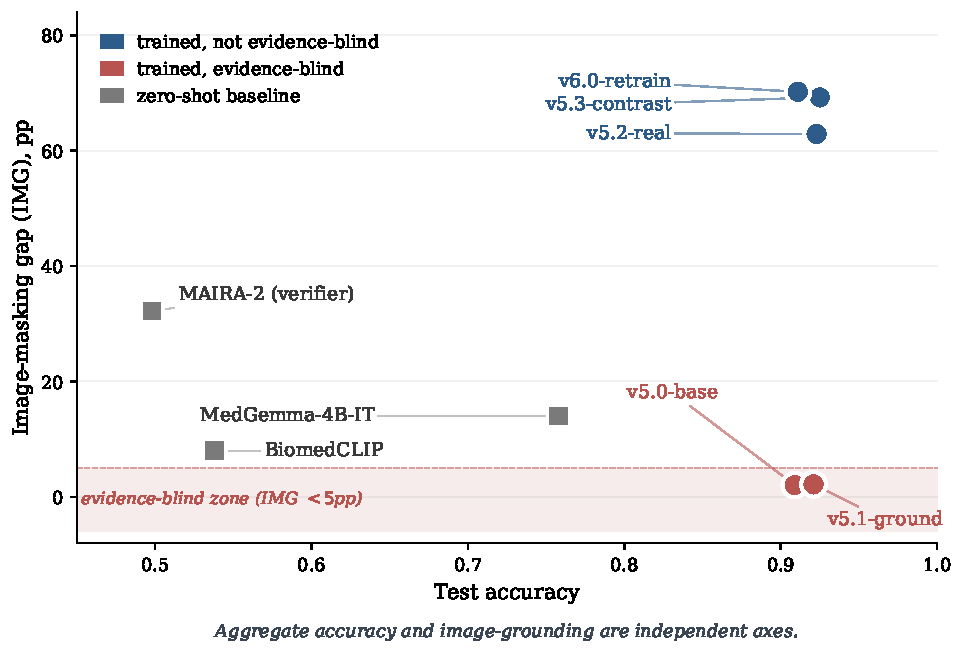
\includegraphics[width=\linewidth]{figures/F2_decoupling_scatter.pdf}
\caption{\textbf{Aggregate accuracy and image-grounding are independent axes.} Circles: trained configurations. Squares: zero-shot detectors on the $500$-claim real-RRG subset. Shaded band: evidence-blind zone (IMG $<5$pp). v5.0 and v5.1 sit in the blind zone at $90$--$92\%$ accuracy; zero-shot baselines BiomedCLIP and MedGemma-4B-IT are blind on ESG.}
\label{fig:decoupling}
\end{figure}

\paragraph{Field audit on real hallucinations.} Figure~\ref{fig:decoupling} extends the diagnostic to $500$ real-RRG claims for three public detectors. BiomedCLIP zero-shot reaches $0.538$ accuracy with IMG $=8.0$pp and ESG $=0.0$pp (blind on ESG). MedGemma-4B-IT as a verifier reaches $0.758$ with IMG $=14.0$pp and ESG $=2.0$pp (blind on ESG). MAIRA-2 used as a zero-shot verifier clears both thresholds (IMG $=32.2$pp, ESG $=6.6$pp) but at near-chance accuracy. The combination matters: a verifier can fail one axis without failing the other, and aggregate accuracy alone does not predict the joint outcome.

\paragraph{Cross-site regression and deployment alarm.} Two leave-one-site-out configurations trained under the v5.3 loss composition show the mitigation does not transfer (Table~\ref{tab:headline}, bottom). Held-out OpenI regresses to IMG $=3.21$pp (within $1.2$pp of the v5.0 baseline); held-out ChestX-Det10 keeps most of the IMG mitigation but drops to ESG $=2.69$pp, below threshold. The same diagnostic that caught the training-time blindness catches the post-deployment one: this is the second role of the same three metrics.

\paragraph{Conformal selection collapses on blind verifiers.} Wrapping inverted conformal Benjamini--Hochberg around each verifier, only v5.3 produces a populated trusted set at $\alpha = 0.10$: $985$ claims with achieved FDR $0.91\%$ and power $39.6\%$. v5.0, v5.1, and v5.2 collapse to $n_{\text{green}}=0$. The two evidence-blind configurations collapse as expected; v5.2 collapses despite clearing IMG, because the joint distribution of (support score, true label) is not separable enough for BH to find a cutoff below the target level. A conformal guarantee on a blind verifier has nothing to certify; on a near-blind verifier the trusted set also empties.

\section{Limitations and Conclusion}

Three limitations bound our claims. The benchmark spans approximately $7{,}500$ images and $25{,}176$ training claims --- enough to expose evidence-blindness as a measurable failure mode but not to estimate its prevalence at population scale. The training-time mitigation acts on in-distribution shortcuts and is not, on its own, expected to generalize across sites; distribution-shift-aware methods (e.g., weighted conformal inference \citep{tibshirani2019conformal}) are the appropriate tool to extend that closure cross-site, and the diagnostic itself remains the alarm signal in either regime. Laterality-turning claims are insensitive to horizontal flips (IPG within $[-0.88, +0.88]$pp across all configurations) because the consistency loss targets image \emph{presence} rather than spatial arrangement; closing this residual would require an image-encoder-level intervention. All training runs are single-seed; multi-seed replication and PadChest-GR claim-extraction for full three-site training are deferred to an extended version.

We introduced a counterfactual diagnostic for multimodal medical claim verification. The cross-entropy baseline reports $90.9\%$ test accuracy while being image-blind at IMG $=2.03$pp; a consistency loss combined with an adversarial hypothesis-only filter closes the in-distribution gap to $69.24$pp; the same three metrics catch the cross-site regression and predict the conformal trust-set collapse on every blind configuration. Counterfactual evidence-sensitivity testing should precede aggregate-accuracy reporting and conformal trust-selection for any multimodal medical verifier; benchmark maintainers and submission checklists should report partial-input baselines alongside aggregate accuracy, as the NLI community did after \citep{gururangan2018annotation,poliak2018hypothesis}.

{\setlength{\bibsep}{0.3em}
\footnotesize
\bibliographystyle{abbrvnat}
\bibliography{sample}}

\end{document}
